\label{ch:approach}

This chapter presents the contribution of this work, first in a generalized form and later with details specific to our implementation.

\section{WINDL - A Novel Approach To Wind Turbine Control With RL}
\label{section:approach-theory}

\begin{summary}
We present \acf{WINDL}. This section introduces an abstract view of our framework. Main design choices were made regarding the reinforcement learning algorithm, the pre- and post-processing pipeline, and reward shaping. Furthermore, we outline our training process and evaluation methods.
\end{summary}

The fundamental interaction cycle of reinforcement learning (see Figure \ref{fig:rlcycle}) assumes a direct link between the environment and the agent. While it would be mathematically possible to directly feed simulation outputs into the reinforcement learning algorithm and vice versa, we found this to be infeasible in practice. Hence, we introduce a pre- and postprocessing architecture to facilitate learning.

The high-level architecture is described in Figure \ref{fig:high-level-schema}. A wind turbine \textit{simulation} (see Section \ref{section:approach-simulation}) outputs sensor data for every time step, which is fed into a \textit{preprocessing pipeline} (see Section \ref{section:approach-preprocessing}). The output of this pipeline is a state vector and a reward signal (see Section \ref{section:approach-reward-shaping}) which is used as a neural network input in the \textit{agent}. The agent is trained within the \textit{RL algorithm} (see Section \ref{section:approach-rl-algorithm}) to optimize reward. The agent output actions in the Coleman transformed space which are processed to pitch angles in the \textit{postprocessing pipeline} (see Section \ref{section:approach-postprocessing}). These pitch angles are used, together with assistive control actions, as a simulation input (see Section \ref{section:approach-simulation}). From there, the cycle restarts.

\begin{figure}
  \centering
    \begin{tikzpicture}
      \node (sim) [process] {Simulation};
      \node (pre) [process, above right = 0.5cm and 2.5cm of sim] {Preprocess};
      \node (agent) [process, below right = 0.5cm and 2.5cm of pre] {Agent};
      \node (post) [process, below right = 0.5cm and 2.5cm of sim] {Postprocess};

      % \draw [arrow,out=90,in=180] (sim.north) to node[left]{action $a$} (pre.west);
      \draw [arrow] (sim.north) |- node[pos=0.7,above] {$\spitchx_{1-3}, \soopbend_{1-3}, \srot, \spow, \sazi, \stbend_{x,y}$} (pre.west);
      \draw [arrow] (pre.east) -| node[pos=0.25,above] {$s,r$} (agent.north);
      \draw [arrow] (agent.south) |- node[pos=0.75,above] {$a$} (post.east);     
      \draw [arrow] (post.west) -| node[pos=0.25,above] {$\apitchx_{1-3}$} (sim.south);
  
    \end{tikzpicture}
  
    \caption{High-Level schema of \ac{WINDL}}
    \label{fig:high-level-schema}
\end{figure}

\subsection{Preprocessing Simulation States}
\label{section:approach-preprocessing}

\begin{summary}
This subsection describes the preprocessing procedure, which most notably transforms the raw sensor data into a stationary coordinate system through the Coleman transformation and normalizes it.
\end{summary}

Final policy performance is greatly influenced by the quality of pre- and postprocessing of the data. A couple of techniques are common to the entire field of machine learning, like normalization, removal of low quality or unnecessary data and transformations into a format more easily processable for neural networks. Each neural network architecture has slightly different requirements concerning the normalization range, input format, and sensitivity to inaccurate data. Reinforcement learning is no exception to this. However, in contrast to supervised or unsupervised machine learning, pre- and postprocessing can not happen beforehand but has to happen in the sampling loop. We preprocess simulation outputs through the selection of inputs, normalization, a modified Coleman transformation, a Cartesian transformation, and dilated past feeding. 

Wind turbine simulations naturally offer a high number of measurement signals, however on a real wind turbine, the number of sensors is limited due to cost and complexity considerations. For our algorithm, we chose to include the following inputs, which are already measured on most modern turbines:
\begin{itemize}
  \item Rotor speed $\srot$
  \item Generator power $\spow$
  \item Pitch angles $\spitchx_{1-3}$
  \item Out of plane blade root bending moments $\soopbend_{1-3}$
  \item Tower bottom bending moment in wind direction $\stbendx$  
  \item Tower bottom bending moment orthogonal to wind direction $\stbendy$
  \item Azimuthal position of the rotor $\sazi$
\end{itemize}

These values are used as an input to the preprocessing pipeline. Note that we do not utilize wind speed as a signal, as obtaining this is notoriously hard. Anemometers on top of the wind turbine are in the wake effect of the rotor and thus do not give sensible measurements. Furthermore, measuring a single point on the rotor plane with an anemometer does not give much insight into the state at other points on the rotor plane, especially in turbulent winds with strongly local turbulence effects. Through the use of neural networks, including more sophisticated sensor arrays such as LIDARs or local blade inflow measurements is possible, but remains open to future work. 

\begin{figure}
  \centering
  \begin{tikzpicture}
    \node (cartesian) [process] {Cartesian Transform};
    \node (coleman) [process, below = 2cm of cartesian] {Coleman Transform};
    \node (normalization) [process, below right = 0.5 and 0.5cm of cartesian] {Normalization};
    \node (past) [process, right = 1.5cm of normalization] {Dilated Past Feeding};
    \node (reward) [process, below = 2cm of normalization] {Reward};

    \coordinate [left = 1.5cm of cartesian.west] (cartesianin);
    \coordinate [left = 1.5cm of coleman.west] (colemanin);
    \coordinate [left = 5.25cm of normalization.west] (normalizationin);
    \coordinate [left = 5.25cm of reward.west] (rewardin);
    \coordinate [right = 1cm of past.east] (pastout);
    \coordinate [right = 5.75cm of reward.east] (rewardout);

    \draw [arrow] (cartesianin) to node[above]{$\sazi$} (cartesian.west);
    \draw [arrow] (colemanin) to node[above]{$\soopbend_{1-3}$}(coleman.west);
    \draw [arrow] (normalizationin) to node[above]{$\spitchx_{1-3}, \soopbend_{1-3}, \srot, \spow, \stbend_{x,y}$}(normalization.west);
    \draw [arrow] (rewardin) to node[above]{$\spitchx_{1-3}$} (reward.west);
    \draw [arrow] (past.east) to node[above]{$s$} (pastout);
    \draw [arrow] (cartesian.east) -| node[pos=0.25,above]{$\cartazix, \cartaziy$} (normalization.north);
    \draw [arrow] (coleman.east) -| node[pos=0.25, above]{$\tilde{c_s}, c_d, c_q$} (normalization.south);
    \draw [arrow] (coleman.east) -| (reward.north);
    \draw [arrow] (normalization.east) to node[above]{$s_{comp}$} (past.west);
    \draw [arrow] (reward.east) to node[above]{$r$} (rewardout);

  \end{tikzpicture}

  \caption{Preprocessing pipeline}
  \label{fig:preprocessing-pipeline}
\end{figure}

Figure \ref{fig:preprocessing-pipeline} shows the components of the preprocessing pipeline. Bending moments $\soopbend_{1-3}$ and azimuth angle $\sazi$ are transformed to a more suitable coordinate system and added back to the state vector. Then, the entire state vector is fed through a normalization component to make the input suited for gradient computation through backpropagation. The normalized outputs are then enriched with information from past steps to ensure the Markov property before they are fed to the neural network. The reward function utilizes information from the transformed bending moments and the pitch angles and is a heuristic for blade and pitch wear.

More precisely, we employ a Coleman Transformation for the bending moments as noted in Equation \ref{eq:coleman-forward}. $c_d$ and $c_q$ are concatenated to the state space, while $c_s$ is highpass-filtered to $\tilde{c_s}$ before concatenation. Furthermore, the untransformed bending moments are part of the state space as well, as this redundant inclusion of transformed and untransformed moments improved performance empirically. We transform the rotor azimuth to Cartesian coordinates on a unit circle and concatenate $\cartazix$ and $\cartaziy$ to the state space. Here, using the untransformed azimuth angle did not play out favorably, so it is dropped from the state vector. As simulation outputs are several orders of magnitude away from each other, we employ a running normalization which we seed with pre-computed values from past runs. We normalize to mean 0 and standard deviation 1 on all input signals. As the state space does not fulfill the Markov property, we employ the trick from \citet{mnihPlayingAtariDeep2013} of concatenating past states to the current one. Improving upon this, we employ a technique which we call \textit{dilated past feeding}. The 15-element state vector $s_{comp}$, which is output by the normalization process, is shown in Equation \ref{eq:state-vector}:

\begin{equation}
  s_{comp} = \text{norm} \left(
  \begin{bmatrix}
    \srot &
    \spow &
    \spitcha &
    \spitchb &
    \spitchc \\
    \soopbenda &
    \soopbendb &
    \soopbendc &
    \stbendx &
    \stbendy \\
    \tilde c_s &
    c_d &
    c_q &
    \cartazix &
    \cartaziy
  \end{bmatrix} 
  \right) \in \mathbb{R}^{15}
  \label{eq:state-vector}
\end{equation}

with $\srot$ being the current rotational speed, $\spow$ the current output power, $[\spitcha, \spitchb, \spitchc]$ the measured pitch angles from the simulation, $[\soopbenda, \soopbendb, \soopbendc]$ the out-of-plane bending moments, $[\stbendx, \stbendy]$ the tower bottom bending moments along and orthogonal to the wind direction, $[\tilde{c_s}, c_d, c_q]$ being the output of the modified Coleman transformation and $[\cartazix, \cartaziy]$ being the azimuth angle $\sazi$ in a Cartesian coordinate system. The final state vector $s$ after dilated past feeding has a dimension multiple of 15, as past feeding concatenates copies of this vector from different points in the past together.

\subsubsection{Cartesian Transformation}

The raw azimuth angles from the simulation form a sawtooth pattern, which linearly rises from 0 to 360 degrees and then drops back to zero in one timestep. This means there is a large difference between the azimuth input for 359 and 1 degree, albeit the actual difference in rotor position is minimal. To give a smoother input, we transform the azimuth to cartesian coordinates on a unit circle with $\cartazix = \sin(\sazi)$, $\cartaziy = \cos(\sazi)$ and drop the raw azimuth angle.

\subsubsection{Normalization}

Using a normalization improves backpropagation performance. Mathematically it is not necessary as the first-layer weights could perform any normalization and the gradient calculation process is mathematically independent of the range of input values. However, experience has shown that the backpropagation algorithm performs better with normalized values as gradient errors are dependent on the magnitude of input values and could cancel out effective gradient updates. 

For some architectures like ResNets, there is a fixed normalization target, to which inputs should be normalized to. To our knowledge, no strict normalization targets are established for the fully connected network in use in our work. Hence, we choose to normalize to mean 0 and standard deviation 1.

We use a running normalization to continuously update our normalization parameters to match the stream of observations that is being fed in through the pipeline. The longer the training runs, the smaller the step size with which we update our normalization to avoid interfering with the learning process. To avoid strong updates at the beginning, we seed our normalization with precomputed parameters.

Welford's algorithm \cite{welfordNoteMethodCalculating1962} for estimating both means and variances in one pass is numerically stable and can calculate a running normalization. The running mean is computed intuitively like Equation \ref{eq:welford-mean}:

\begin{equation}
  \bar{x}_n = \bar{x}_{n-1} + \frac{x_n - \bar{x}_{n-1}}{n}
  \label{eq:welford-mean}
\end{equation}

with $x_n$ being the original signal at sampling point $n$, and $\bar{x}_n$ the estimation of the running mean at sampling point $n$. The running variance estimation works by keeping a sum of squared differences $\mathcal{M}_{n}$ as in Equation \ref{eq:welford-sum}:

\begin{equation}
  \mathcal{M}_{n} = \mathcal{M}_{n-1} + (x_n + \bar{x}_{n-1})(x_n - \bar{x}_n)
  \label{eq:welford-sum}
\end{equation}

with this sum, the Bessel-corrected standard deviation estimate $\sigma$ can be computed as ${\sigma_n}^2 = \frac{\mathcal{M}_{n}}{n-1}$. Sampling is done across all rollouts, i.e. $n$ increases monotonically even across environment resets. To give reasonable normalization on the first samples, we seed $\bar{x}$ and $\mathcal{M}_{n}$ to values computed from previous trainings and set $n=1\text{e}6$ at the beginning of the training. To prevent $n$ and $\mathcal{M}_{n}$ from reaching infinity, we stop the algorithm and freeze mean and standard deviation estimates when $n>10^8$. Equation \ref{eq:normalization} normalizes input values to mean 0 and standard deviation 1:

\begin{equation}
  \text{norm}(x_n)= \text{clip}_{\pm 5} \left( \frac{x_n - \bar{x}_n}{\sigma_n} \right)
  \label{eq:normalization}
\end{equation}

We employ observation clipping to prevent strong outlier values from reaching the neural network, as this induces gradient instability.

\subsubsection{Modified Coleman Transform}

We utilize a Coleman transformation of the bending moments for preprocessing with an addition of a highpass filter on the first component. This transformation projects the rotating coordinate system of the blades to a blade-invariant fixed coordinate system across the rotor plane. As the blades are symmetric, they exhibit the same behavior when at the same point in the rotor plane. Through the Coleman transformation, the reinforcement learning algorithm does not have to learn the mechanics of the wind turbine for each blade separately and can learn the mechanics across the rotor plane at once instead.

The Coleman transformation is used as described in Equation \ref{eq:coleman-forward}. It takes the three bending moments and the azimuth angle as input and outputs three variables $(c_s, c_d, c_q)$. $c_d$ is the difference in moments at the top and the bottom of the rotation, acting as a tilting force. $c_q$ acts similarly but in a yawing direction. $c_s$ is the mean offset component of the bending forces. When wind hits the rotor, bending moments are always highly positive, hence $c_s$ is always highly positive and offers a poor signal-to-noise ratio. The presence of the offset itself is not surprising and can be considered noise, we are instead interested in \textit{changes} in bending moments. These changes could result in tower vibrations, blade vibrations, or other damaging effects. Thus, we employ a highpass filter to $c_s$ obtaining a filtered signal $\tilde c_s$ without the constant component. Our highpass-filter is implemented as a first-order discrete highpass filter as described in Equation \ref{eq:coleman-highpass}:

\begin{equation}
  \tilde c_{s,t} = \frac{-(\Delta t - 2 \tauhp )\tilde c_{s, t-1} + 2\tauhp c_{s,t} - 2\tauhp c_{s, t-1}}{ \Delta t + 2\tauhp }
  \label{eq:coleman-highpass}
\end{equation}

with $c_{s, t}$ being the $c_s$ signal at timestep $t$, $\Delta t$ the simulation time step size and $\tauhp$ the highpass filter constant. We set $\tauhp$ to $\frac{1}{0.2}$ to filter out frequencies below 0.2 Hertz, which is roughly equal to the turbine rotation frequency. The three variables $\tilde c_s$, $c_d$ and $c_q$ are concatenated to the state space, the unfiltered $c_s$ is discarted.

\subsubsection{Dilated Past Feeding}

We introduce a technique, which we call \textit{dilated past feeding}, to fulfill the Markov property for our state space by efficiently feeding a large stack of past states without requiring a recurrent neural architecture. The Markov property means that the next state only depends on the previous one, not on anything before. In practice, this is not the case for the wind turbine environment. For example, the beginning of a gust could look quite similar to the end of a gust in terms of rotor speed, power, and loads. However, before a gust, loads are bound to increase, while after a gust, they decrease. These scenarios require drastically different control actions. Additional information from states from the past can help to determine more accurately the state in which the turbine is in. Hence, we concatenate past observations to each state with a large enough time window, so everything before that window only has a minor impact on the next state, similar to \citet{mnihPlayingAtariDeep2013}. 

For the wind turbine environment with its high inertias, the time frame of inertial activity is prohibitively large for traditional past feeding, hence we use dilated past feeding as an improved version of past feeding which reduces input dimensionality. Equation \ref{eq:dilated-past-math} describes the procedure:
\begin{equation}
 s_t \cdot f(1, t) \cdot f(2, t) \cdot ... \cdot f(\lambdapast, t)
\label{eq:dilated-past-math}
\end{equation}

with $\cdot$ being the concatenation operator and $f(i, t)$ as defined in Equation \ref{eq:dilated-past-mathf}

\begin{equation}
\left. f(i, t) = \frac{1}{t_1 - t_0}\sum^{t_1}_{t=t_0} s_t \right| t_0 = t-\frac{i(i+1)}{2}, t_1 = t-\frac{(i+1)(i+2)}{2} - 1
\label{eq:dilated-past-mathf}
\end{equation}

$f(i, t)$ averages across an increasing number of past states, reducing more and more states into one. An intuition for this averaging operation is given in Equation \ref{eq:dilated-past-intuition}:

\begin{equation}
\underbrace{s_t}_{s_t},\: \underbrace{s_{t-1},\: s_{t-2}}_{f(1,t)},\: \underbrace{s_{t-3},\: s_{t-4},\: s_{t-5}}_{f(2,t)},\: \underbrace{s_{t-6},\: s_{t-7},\: s_{t-8},\: s_{t-9}}_{f(3,t)},\: ...
\label{eq:dilated-past-intuition}
\end{equation}

This way, information about a high number of past states can be passed to the network with a small increase in neural network input dimensionality. More recent states are averaged across shorter time-spans and thus retain more information, while more distant states are averaged across a longer time span. Loosing some information from states further in the past is less critical, as small deviations are unlikely to play out as strong as the general direction of change. The dimensionality reduction is significant, for example with a value of $\lambdapast = 6$, information from 28 states is combined to a resulting dimension of just seven times the original state dimension. Furthermore, the averaging operation counteracts spatial noise, giving a more stable view into the operating state of the turbine in the near past.

It would be imaginable to utilize a recurrent neural architecture such as a LSTM \cite{hochreiterLongShortTermMemory1997} to allow looking at large sequences of past states instead of using dilated past feeding. A more complex architecture also comes with more failure conditions like susceptibility to vanishing and exploding gradients. Our dilated past feeding encodes the intuition that recent states are more important than states far in the past, which the LSTM would have to specifically encode into its forget-gates. Also, the LSTM would not perform smoothing over past states, which we believe to be a positive contributing factor over past states. For an application to more complex sensor-arrays like LIDAR which already bring a high dimensional input, we could imagine a convolutional recurrent neural network to be a good choice, but in our case we found dilated past feeding to be sufficient.

\subsection{Postprocessing Actions}
\label{section:approach-postprocessing}

\begin{summary}
This subsection introduces the postprocessing pipeline, which most notably transforms actions from the stationary Coleman space into individual pitch actions and integrates an assistive \ac{CPC}.
\end{summary}

The post-processing procedure aims to improve training stability and facilitate learning. There are some requirements to the post-processing pipeline: The output range should be compatible with the activation function, the room for erratic actions should be minimal without limiting the room for sensible actions, and output dimensionality and complexity should be as low as possible. We aim to fulfill these requirements through three techniques: (de)normalization, the Coleman Backtransform, and an assistive CPC controller.

\begin{figure}
  \centering
  \begin{tikzpicture}
    \node (normalization) [process] {Denormalization};
    \node (coleman) [process, left = 1cm of normalization] {Coleman Backtransform};
    \node (plus) [joiner, left = 2cm of coleman.west] {$+$};
    \node (cpc) [process, below = 1cm of coleman] {CPC};

    \coordinate [right = 1cm of normalization.east] (normalizationin);
    \coordinate [left = 1cm of plus.west] (simout);

    \draw [arrow] (normalizationin) to node[above]{$a$} (normalization.east);
    \draw [arrow] (normalization.west) to node[above = 0.5cm]{$c_D, c_Q, \philead$} (coleman.east);
    \draw [arrow] (coleman.west) to node[above]{$\apitchxd_{1-3}$} (plus);
    \draw [arrow] (cpc.west) -| node[pos=0.25,above]{$\apitch$} (plus);
    \draw [arrow] (plus.west) to node[above]{$\spitchx_{1-3}$} (simout);

  \end{tikzpicture}

  \caption{Postprocessing pipeline}
  \label{fig:postprocessing-pipeline}
\end{figure}

A schema of our pipeline is shown in Figure \ref{fig:postprocessing-pipeline}. The raw neural network output $a$ is fed into a denormalization component, which brings actions from a range of $[-1, 1]$ to the range required for the next component, the Coleman Backtransform. There, the inverse Coleman Transformation is applied to the inputs, yielding three pitch signals. These pitch signals are then added to an assistive collective pitch output from a traditional CPC and fed into the simulation.

\subsubsection{Denormalization}

In contrast to the normalization in the preprocessing pipeline, the output denormalization is a static multiplication and offset. Neural network outputs are denormalized from a range of $\pm1$, which is the range of the activation function in use, to the ranges necessary in the Coleman Backtransform. 

The resulting normalized action space on the neural network side has the three elements from Equation \ref{eq:action-vector}.

\begin{equation}
  a = \text{norm} \left(
  \begin{bmatrix}
    c_D & c_Q & \philead
  \end{bmatrix} 
  \right) \in (-1, 1)^3
  \label{eq:action-vector}
\end{equation}


\subsubsection{Coleman Backtransform}

Working in the Coleman domain enables the agent to output azimuth-independent control signals, and as such, makes the output space less complex. An action in the Coleman space will always have the same result, indifferent of which individual blade is executing it. This idea takes inspiration from the design of Coleman-based IPC control strategies, which use the same methodology.

The state of the inflowing wind can be locally different in different parts on the rotor plane. If one blade just hit a strong gust close to the ground, the next blade is likely going to encounter the same gust when it arrives at the same point of the rotation. This is especially true for modern large wind turbines, which span a large rotor area with much space for locally different wind inflow. Outputting actions in the rotation invariant Coleman space, the neural network can detect such a local gust and apply a counteraction on that specific location of the rotor plane, without caring for which individual blade is currently passing that location. 

The Coleman Backtransformation as described in Equation \ref{eq:coleman-backward} transforms from rotation independent values to blade specific ones. The transformation takes the values $[c_S, c_D, c_Q, \philead]$ as input and outputs individual pitch offsets $[\apitchad, \apitchbd, \apitchcd]$. As with the forward transformation, $c_S$ can be understood as a collective offset of all pitch angles towards the baseline pitch signal. $c_D$ is equal to a tilting difference in pitch - if it is positive, transformed pitch values are positive in the upper half of the rotation and negative in the lower half. $c_Q$ obeys the same principles but in the yawing direction. 

The range of input values depends on the freedom the RL agent should have. If the desired maximum offset from the \ac{CPC} signal is $\pm \ipcplay$ degrees, the input range to the Coleman Backtransformation should be limited to $\pm \frac{\ipcplay}{\sqrt{2}}$. A typical value for $\ipcplay$ in PID-based controllers is $\pm4$ deg. $\philead$ determines a lead angle in the azimuth calculation. This can be understood as a rotation of the axes along the rotor plane that $c_D$ and $c_Q$ act on. $\philead$ could theoretically take on any value from $-\cpi$ to $\cpi$ rad, which would allow the controller to flip the transformed coordinate system completely. To retain interpretability, we restrict it to $\pm\frac{1}{4}\cpi$ rad. We observed adverse effects between the \ac{RL} controller and the \ac{CPC} if $c_S$ is used extensively by the agent. Hence, we set $c_S=0$ unless stated otherwise and do not make it part of the action space.

\subsubsection{Assistive CPC}

A significant requirement to output preprocessing is to exclude as many erratic actions as possible from the action space without limiting sensible actions. To achieve this, we utilize an assistive CPC controller to output a sensible average pitch action based on a proven control strategy, from which the reinforcement learning controller can deviate away in a safe range. This range can be chosen to be large enough to allow for a significant improvement over the CPC action, but not large enough to induce fatal turbine damage through erratic actions. With this assistive formulation, even a poor policy does not have the potential to destroy the turbine, which would complicate learning. Furthermore, if the network outputs all zeros (no deviation), the baseline CPC action will be applied without changes and safely keep the turbine operational.

More formally, the CPC outputs a collective pitch action $\apitch$, which is used to calculate the final individual blade pitch actions by adding individual pitches: $\apitchx_{1-3} = \apitch + \apitchxd_{1-3}$. We use the \ac{CPC} policy as described in Section \ref{section:background-cpc} and which also forms one of our evaluation benchmarks. The individual pitch actions $\apitchxd \in \pm \ipcplay$ are limited to a safe pitch range, with the range hyperparameter $\ipcplay$ subject to hyperparameter tuning. In the IPC baseline, a range of $\ipcplay=4$ is used.


\subsection{RL Agent}
\label{section:approach-rl-algorithm}

\begin{summary}
This subsection discusses considerations and changes concerning the reinforcement learning algorithm. We choose \ac{SAC} \cite{haarnojaSoftActorCriticOffPolicy2018} as our reinforcement learning algorithm due to good overall performance, sample efficiency, and the ability to control the exploration-exploitation trade-off. Furthermore, we implement a smoothness regularization to make it more suited to control a noise-susceptible wind turbine.
\end{summary}

The envisoned life cycle for our controller is to train a policy once, which is able to handle all sorts of weather conditions, and let it run in inference mode on the real-world turbine for the rest of its lifetime. When operating conditions deviate from what the policy was trained on, the supervisory control would switch to a different control strategy, which can deal with the weather scenario. We do not envision online training on the turbine due to safety concerns. To reflect this, all evaluation runs are executed without updating the policy. Because we do not envision training on the turbine, it is feasible to run a compute-intensive training. Practically, limitations for computational budget or development time might apply especially to small wind turbine models, so an algorithm should deliver high performance and robustness while showing reasonable sample efficiency.

We utilize the reinforcement learning algorithm \acl{SAC} by \citet{haarnojaSoftActorCriticOffPolicy2018} with the improvements from their follow-up paper \cite{haarnojaSoftActorCriticAlgorithms2019} and smoothness regularization \cite{mysoreRegularizingActionPolicies2021} as described in Section \ref{section:background-sac}. The algorithm optimizes the maximum entropy objective from Equation \ref{eq:soft-policy-objective}. 

This algorithm is an off-policy algorithm, meaning it can learn from experience in a replay buffer. This makes it more sample efficient than other on-policy algorithms like \ac{PPO} \cite{schulmanProximalPolicyOptimization2017}, reducing the amount of computation time necessary. Furthermore, it exhibits more training stability, and hyperparameter insensitivity than other off-policy algorithms like \ac{TD3} \cite{fujimotoAddressingFunctionApproximation2018}. However, in final policy performance it matched or outperformed other competitors. 

Our policy network is a fully connected \ac{MLP} without layer- or batch-normalization. The output is a multivariate Gaussian of the dimensionality of the action space $A$, with both the mean and standard deviation being network outputs. The covariance matrix is diagonal, hence the mean and standard deviation outputs have the same length. For the standard deviation we utilize exponential parametrization, i.e. the last layer outputs for the standard deviation portion are exponentiated. The Q-function networks are fully connected \acp{MLP} without layer- or batch-normalization. Q-function and policy networks do not share weights.

Gradient updates are performed according to the Adam strategy \cite{kingmaAdamMethodStochastic2017} with different learning rates for policy and Q-function. The beta parameters are set to their default values of 0.9 and 0.999, and no L1 or L2 norm is applied to the weights.

Furthermore, we utilize the smoothing regularization from \citet{mysoreRegularizingActionPolicies2021} with euclidean distances for both temporal and spatial regularizations as described in Section \ref{section:background-smoothness-regularization}. The perturbation for the spatial regularization is a spherical gaussian.

% When stated, we utilize the value regularization from \citet{kumarDR3ValueBasedDeep2021} as described in Section \ref{section:background-value-regularization}. As \ac{SAC} does not use next actions in the Q-function update, next actions are not already sampled from the replay buffer. Instead of modifying the sampling procedure from the replay buffer, we adjust the regularization slightly to sample the next action from the policy instead, as shown in Equation \ref{eq:dr3-regularization-adjusted}:

% \begin{equation}
%   \drrrreg = \drrrcoeff \frac{1}{|D|} \sum_{s_t, a_t, s_{t+1} \backsim D, a_{t+1} \backsim \pi(s_{t+1})} \qlastlayer(s_t, a_t)^\intercal \qlastlayer(s_{t+1}, a_{t+1})
%   \label{eq:dr3-regularization-adjusted}
% \end{equation}

% This $a_{t+1}$ is already present in the SAC update and requires minimal changes to the code.

\subsection{Reward Shaping}
\label{section:approach-reward-shaping}

\begin{summary}
This subsection introduces our reward function and what considerations lead to its design. It consists of a blade penalty part, a pitch penalty part and a constant offset.
\end{summary}

Reward shaping is crucially important to the success of reinforcement learning, as this is the bridge between the abstract goals of the human engineer and the mathematical quantity that is being optimized. Effectively, the engineer is optimizing \acf{LCOE} - the end-to-end costs of producing a fixed amount of electric energy. However, the complete process from wind turbine design to operation is way too complex to be directly optimized by a reinforcement learning algorithm. For the small subfield of wind turbine load control, multiple optimization aims are in place as described in Section \ref{section:background-optimization-aims}. We mainly focus on pitch wear and blade wear and incorporate heuristics for these into our reward function.

The requirements for a good reward function are manifold. First and foremost, it shall represent the optimization aims. It shall not exhibit local maxima, which could lead the agent to unwanted behavior. A reward signal each time step is easier to learn than a sparse reward at the end of a trajectory, so there should be a reward signal for each time step. And lastly, the signal-to-noise ratio in the reward signal should be as high as possible, excluding irrelevant deviations. The reward function we utilize is outlined in Equation \ref{eq:reward-function}

\begin{equation}
  % r(s,a) = \text{clip}_{\pm 5}(-\rcoleman \sqrt{\tilde { + }c_d^2 + c_q^2} - \rpitchtravel (\frac{1}{3}\sum_{i \in [1,2,3]} | \partial \spitchx_{i} |) + \rconst) 
  r(s,a) = \text{clip}_{\pm 5}(-\rcoleman \sqrt{\tilde{c_s}^2 + {c_d}^2 + {c_q}^2} - \rcolemanact \sqrt{{c_S}^2 + {c_D}^2 + {c_Q}^2} + \rconst)
  \label{eq:reward-function}
\end{equation}

The Coleman based reward function in Equation \ref{eq:reward-function} is inspired by the design goals of a Coleman Transformation based \ac{IPC}. The norm of the vector $[\tilde c_s, c_d, c_q]$ serves as a heuristic for blade wear and is scaled with a factor $\rcoleman$. Higher values of $\rcoleman$ will mean a higher penalty for blade wear. The norm of the vector $[c_S, c_D, c_Q]$ is a heuristic for pitch wear and scaled by $\rcolemanact$. 

The first half of the reward function, the norm of the vector $[\tilde c_s, c_d, c_q]$, is inspired by the error term for the PID controllers in an IPC. An \ac{IPC} after \citet{bossanyiFurtherLoadReductions2005} contains PID controllers trying to bring $c_d$ and $c_q$ to zero by outputting respective $c_D$ and $c_Q$ signals. We furthermore add $\tilde c_s$ because of a flaw in this cost function. Minimizing $c_d, c_q$ alone minimizes the \textit{difference} in bending moments across the rotor plane. A possible exploit to this is to keep this difference small, but have the \textit{mean} of the bending moments oscillate, swinging the entire turbine back and forth. The traditional \ac{IPC} does not know how to exploit that weakness in the reward function, but we found RL agents to be capable of finding and using this flaw. To counteract this, the highpass-filtered $\tilde c_s$ signal is introduced as well. A swinging turbine will induce collective blade loads, which will yield a $\tilde c_s$ based penalty.

The vector $[c_S, c_D, c_Q]$ in the second half of the reward function is just the neural network output, excluding $\philead$. The further away from zero $c_D, c_Q$ are, the higher the IPC activity across the respective axis of the rotor plane. Penalizing the norm of this incentivizes low pitch activity. Furthermore, including $c_S$ keeps the controller from reducing thrust excessively. A high value of $c_S$ induces a positive constant offset to all pitch angles, reducing overall rotor thrust at the expense of power. Because we did not explicitly model power into our reward function to simplify learning, we incentivize the controller to deviate from the assistive CPC action as little as possible.

The factors $\rcoleman, \rcolemanact$ are also used to scale the rewards to lay between 0 and 1. Though theoretically not necessary as it does not move the maxima, in practice, it is easier to learn a reward function between 0 and 1. Otherwise, the outputs of the Q function are too high for accurate approximation through a neural network. To prevent excessively large values which could induce learning instability, we clip the reward to $\pm 5$. 

% To be able to limit excessive pitch activity, a penalty for pitch travel is introduced with the constant factor $\rpitchtravel$. By setting a positive $\rpitchtravel$, the difference in pitch between the current and last time step $\partial \spitchx_{i} = \spitchx_{i, t} - \spitchx_{i, t-1}$ averaged across all blades $i \in [1,2,3]$ is subtracted from the reward. Together with the CAPS parameters, this reward coefficient can be used to control the pitch-blade tradeoff (see Section \ref{section:results-pb-trade-off}).
% Requiring the last pitch angle to compute the current reward breaks the Markov-Property for reward functions and thus breaks one of the assumptions for the theoretical proof of the \ac{SAC} algorithm, hence we use $\rpitchtravel = 0$ wherever possible. However, we found it to work well in practice. 
$\rconst$ is a constant offset that is added to the reward at every step. This prevents another exploit in the reward function. Reinforcement learning optimizes expected accumulated return. Accumulating a lot of negative rewards leads to a largely negative return. Through extremely erratic actions, the controller has the ability to destroy a turbine even despite safety margins in place. Ending an episode through turbine destruction induces a period of highly negative rewards when the turbine is almost destroyed but not completely. This highly negative period can have a better return in sum due to the episode ending early, and as such, becomes the global maximum. To prevent such suicidal behavior, we aim for mostly positive rewards.

We found the Coleman-based reward function to meet our requirements of being easy to optimize - as it is directly computed as a 2-norm of observations and actions, a Q-function approximator has less barrier in learning this reward function, and predicting future rewards is the main focus. Local maxima in suicidal behavior, swinging the turbine back and forth, and reducing power yields are inhibited through countermeasures. And in contrast to other choices like optimizing \acp{DEL} (which can only reasonably be computed at the end of a trajectory), this reward function gives relatively instantaneous feedback to good or poor actions. 


\subsection{Simulation Wrapper}
\label{section:approach-simulation}

\begin{summary}
This subsection describes the wrapper around the simulation tool, which includes an assistive control system for torque control and the pitch actuator model. Furthermore, we present the reference turbine used in this work, a 10MW offshore turbine.
\end{summary}

The wind turbine simulation is at the heart of the environment, simulating the underlying turbine, controller, and wind interaction. We add assistive controllers to mask away side problems irrelevant to the actual reinforcement learning aim of load reduction. Furthermore, we discuss considerations for a pitch actuator model, as our choice of simulation does not bring its own pitch actuator model at the time of writing. This subsection describes considerations independent of the actual choice of simulation tool, while Section \ref{section:approach-qblade} goes into detail on the specific tool in use in this work.

\begin{figure}
  \centering
  \begin{tikzpicture}
    \node (sim) [process] {IEA-10MW Simulation};
    \node (model) [process, below = 1cm of sim.south] {Pitch Actuator Model};
    \node (assist) [process, right = 3cm of sim.east] {Assistive Control};

    \coordinate [above = 1cm of sim.north] (simout);
    \coordinate [below = 1cm of model.south] (simin);

    \draw [arrow] (simin) to node[right]{$\apitchx_{1-3}$} (model.south);
    \draw [arrow] (model.north) to node[right]{$\spitchx_{1-3}$} (sim.south);
    \draw [arrow] (assist.west) to node[above]{$T, \ayaw$} (sim.east);
    \draw [arrow] (sim.north) to node[right]{$\spitchx_{1-3}, \soopbend_{1-3}, \srot, \spow, \sazi, \stbend_{x,y}$} (simout);

  \end{tikzpicture}

  \caption{A wrapper around the simulation}
  \label{fig:simulation-wrapper}
\end{figure}


Figure \ref{fig:simulation-wrapper} describes the components which wrap around our simulation tool. A pitch actuator model simulates the dynamics of the pitch motors, pitch bearings, and inertias related to pitching actions. To mask away torque and yaw control, we utilize assistive control systems for these required control signals. The simulation itself simulates the IEA-10MW offshore turbine.

\subsubsection{IEA-10MW Wind Turbine}

We perform our experiments on the IEA 10MW wind turbine model by \citet{bortolottiIEAWindTCP2019}. The IEA 10MW is a large offshore wind turbine with a blade length of 96 m and a hub height of 119 m. It has a rated wind speed of 10.75 m/s at a rated rotational speed of 8.68 rpm. With such large turbines, traditional control strategies reach their limitations, and the potential for improvement is larger than with a smaller turbine.

Before switching to RL control, we let the turbine ramp up and settle with a \ac{CPC} controller until no major oscillations are visible in steady state. To reduce blade-specific learning artifacts, we randomized the initial rotor azimuth angle. 

We choose a simulation resolution of 10 simulation steps per second, as with such a high resolution fast reaction times are possible. The simulation is done with the help of a \acf{BEM} method, which is a wind turbine simulation method, which splits the blades into sections and computes each section's lift and drag with simplified formulas. There are approaches, which deliver higher accuracies like the Lifting Line Free Vortex Wake method, but generally, \ac{BEM} methods are well established in wind turbine research and deliver good enough results for our purposes while being computationally cheap.

\subsubsection{Assistive Control Systems}

Our algorithm only tackles pitch control, but the simulation requires a pitch, torque, and yaw signal. Torque and yaw control are different problems out of the scope of this work. To separate concerns, we mask away these control systems from the reinforcement learning agent, so it does not have to learn multiple control systems at once. 

We design our wind fields to always face the front of the wind turbine, which is why the yaw action $\ayaw$ is kept constant at zero and does not require an additional assistive control system. To simulate a slow-reacting yaw controller, we add some horizontal inflow randomization between $\pm8$ degrees. Values outside of that would be corrected quickly by most yaw controllers.

For wind speeds well above rated speed, the torque action $T$ could be kept constantly at its maximum, but for wind speeds below and around rated, and within gusts, the torque might have to deviate. Hence, we utilize an assistive PID-based torque controller to determine torque actions. In traditional control theory, the pitch and torque control systems can not interfere as they are switched over at rated speed. We allow our reinforcement learned pitch controller to also work below rated speeds, which could induce a feedback loop between the two controllers. However, experience shows that if such a feedback loop between the reinforcement learning pitch controller and the torque controller exists, it does not play out harmfully. Hence, we can mask away torque control from the reinforcement learning policy.

\subsubsection{Pitch Actuator Model}
\label{section:approach-actuator-model}

Our simulation does not include a pitch actuator model at time of writing. The pitch values from the controller are directly fed into the structural model without taking into account any inertias, torsional moments, or actuator limitations. To ensure simulation flexibility, controller implementations typically bring their own pitch actuator model \cite{perez-beckerImplementationValidationAdvanced2021} \cite{hansenBasicDTUWind2013}. 

We implement a second-order low-pass filter after \citet[Appendix B.2]{hansenBasicDTUWind2013} to model each blade pitch actuator as in Equation \ref{eq:second-order-lowpass}:
\begin{equation}
  \ddot{\bar{x}} + 2 \pitchmodeldamp \pitchmodelfreq \dot{\bar{x}} + 2 {\pitchmodelfreq}^2 \bar{x} = {\pitchmodelfreq}^2 x
  \label{eq:second-order-lowpass}
\end{equation}
With $x$ being the original, $\bar{x}$ the filtered, and $\dot{x}$ and $\ddot{x}$ being the first and second derivative of the signal $x$. Equation \cite[B.7, B.8]{hansenBasicDTUWind2013} elaborate on how to implement this in a discrete setting. We replace the constants by $\pitchmodelfreq = 4\cpi$ and $\pitchmodeldamp = 0.7$. As the \ac{CPC} controller producing the baseline action brings its own pitch actuator model, we would end up with two actuator models. Consequently, we deactivate any actuator modeling in the \ac{CPC} controller.

\subsection{Wind Scenarios}

\begin{summary}
This section goes into more detail on the parameters for the two wind scenarios \textit{steady wind} and \textit{turbulent wind} that were introduced in Section \ref{section:background-optimization-aims}. During training, the agent sees a different wind speed, inflow angle and turbulent seed on every rollout, while during evaluation, we utilize a fixed set.
\end{summary}

The steady wind setting serves as a test-bed for our trainings, as optimal behavior in this scenario is relatively well researched and predictable. Thus, this scenario offers better possibilities to judge the properties of the trained controller. We do not expect much headroom to improve upon an \ac{IPC} controller in this setting, but if the agent is able to match the performance of an \ac{IPC}, this means training works in principle. Also, the computational requirements of the simulation in the steady wind are lower, as wind field generation is trivial. Hence, we perform bigger parts of our hyperparameter search in this setting. We employ a wind field with a shear coefficient of 0.2, meaning wind speeds at the bottom of the boundary layer are 20\% lower than geostropic wind speeds. The vertical inflow angle is zero degrees, while we randomize horizontal inflow to be either of $\{-8, 0, 8\}$ degrees. We randomize wind speeds and horizontal inflow during training but utilize a fixed set of parameters for evaluation. These fixed parameters allow a direct comparison to the benchmark baselines, and the randomization during training prevents overfit to a predefined set of wind scenarios.

The turbulent wind setting is the setting where we expect more optimization potential compared to traditional IPC methods. However, evaluation of mistakes is more challenging, as it is not clear whether an artifact stems from turbulence or from erratic behavior of the controller. We use a vertical inflow angle of 0 degrees and randomize horizontal inflow to be either of $\{-8, 0, 8\}$ degrees. Our turbulence model is the \acf{NTM} from \citet{internationalelectrotechnicalcommissionIEC61400120192019}, as it is a proven reference model for turbine validation. We use different random seeds for the turbulence generator in every rollout and also uniformly randomize the mean wind speed. As in the steady wind, we only randomize during training and use a set of fixed parameters for evaluation.

\section{Implementation}
\label{section:approach-implementation}

\begin{summary}
In this section, we present implementation details of \ac{WINDL}. The main challenges tackled by the implementation are scalability, efficient experimentation, and the interplay of the various components.
\end{summary}

The requirements for scalability are high in the wind turbine reinforcement learning setting. To train a typical reinforcement learning policy requires something in the order of magnitude from $10^6$ to $10^8$ environment interactions \cite[Figure 3]{haarnojaSoftActorCriticOffPolicy2018} \cite[Methods: Training details]{mnihPlayingAtariDeep2013}. We observed sensible training results after around $2*10^7$ steps. With our simulation tool delivering ca. 70 steps per second on a modern CPU, it would take over three days to collect enough samples for a single training. Additional time spent on updating the neural networks would easily drive total training times to over four days, which is unacceptably high. Increasing the simulation performance would be possible at the expense of accuracy, but to avoid reaching unrealistic behavior and to train on the same settings as we evaluate, we decide against a simplified simulation. Hence, we require parallelization and a high-performance computing cluster to speed up training time without sacrificing accuracy.

We introduce the tools used for simulating, wind field creation, and the controller baseline in Section \ref{section:approach-qblade}. Section \ref{section:approach-cluster} presents the cluster on which we trained, while Section \ref{section:approach-distributed} presents software changes, which enable optimal use of the high computation power of the cluster.

To be able to perform efficient experimentation is fundamental to the success of this work. We want to ensure reproducible results and an insightful evaluation. Section \ref{section:approach-hyperparameters} gives an overview of used hyperparameters and hyperparameter search procedures, and Section \ref{section:approach-evaluation-methodology} describes the detailed evaluation methodology.


\subsection{QBlade Wind Turbine Simulation}
\label{section:approach-qblade}

\begin{summary}
This subsection presents the configuration used for the simulation tools. We use the library interface of QBlade together with TurbSim and the TUBController. 
\end{summary}

We utilize the aeroelastic wind turbine simulation tool QBlade by \citet{martenQBladeModernTool2020}. Compared to other tools such as OpenFAST \cite{buhlOpenFAST}, it offers faster computation at comparable or better accuracy. It can simulate a wide range of turbines, wind inputs, and other simulation options. Other major tools in use are TurbSim \cite{neilkelleyandbonniejonkmanTurbSim} and the TUBController \cite{perez-beckerImplementationValidationAdvanced2021}.

Turbulent wind field generation is performed with the help of the tool TurbSim \cite{neilkelleyandbonniejonkmanTurbSim}, which is part of the OpenFAST repository. Due to its flexibility, we utilize the TUBController \cite{perez-beckerImplementationValidationAdvanced2021} during evaluation for the \ac{CPC} baseline, \ac{IPC} baseline, and during training to compute $\apitch$ for action postprocessing as described in Section \ref{section:approach-postprocessing}. Both the TUBController and TurbSim are integrated into QBlade and implicitly called through the library interface. We compile QBlade, TurbSim, and all of their dependencies with maximal compiler optimizations for the native architecture of the cluster and OpenMP enabled to reach the best possible performance.

QBlade can be compiled to a shared library, which allows the simulation to be embedded into python code via cython. Using the library interface, we develop a python wrapper for the environment. We follow the OpenAI gym interface \cite{brockmanOpenAIGym2016}, a common standard for reinforcement learning environments which is supported by garage. Our python wrapper contains the pre- and post-processing steps outlined in Section \ref{section:approach-preprocessing}, \ref{section:approach-postprocessing}, and \ref{section:approach-reward-shaping} in a pipeline. Due to the pipeline approach, elements of the pipeline can be switched on or off individually. Also, the python wrapper includes the process separating distribution framework as described in Section \ref{section:approach-distributed} and the simulation wrapper as described in Section \ref{section:approach-simulation}.

Especially early in training, the behavior of the reinforcement learning agent can be erratic. Exposed to a real-world turbine, this would lead to immediate turbine damage or destruction. In QBlade, turbine failure is not simulated directly. However, simulation accuracy suffers when the operating conditions exceed a realistic range by a wide margin. Hence, we have to detect extreme situations and terminate a rollout in case unrealistic simulation results are to be expected. The first failure condition is NaN values in the simulation, which happens if the boundary conditions are exceeded by a margin that brings the floating point accuracy to its limits. Furthermore, negative or excessive rotational speeds (50\% higher than rated) are interpreted as turbine failure. Other failure conditions for a real-world turbine, like extreme blade bendings, tower bendings, or a blade hitting the tower are ignored and training continues past such conditions, as the simulation still delivers reasonable results. These states receive a low reward and generally do not occur in later training.

\subsection{Cluster}
\label{section:approach-cluster}

\begin{summary}
This section presents the CPU-only cluster Lise where our computation took place.
\end{summary}

The work was supported by the North-German Supercomputing Alliance (HLRN). We were granted compute time on their cluster Lise. The Lise default nodes are CPU heavy nodes with the following specs:

\begin{itemize}
  \item 2 Sockets Cascade 9242 processors with 48 physical (96 logical) cores each
  \item 362 GB RAM, of which 2-3 GB are used by the operating system and workload manager
  \item No GPUs
  \item 100 GBit/s Infiniband networking
  \item Storage via a network-mounted Lustre file system with up to 85 GB/s streaming bandwidth
\end{itemize}

This CPU focus suits the high CPU requirements of the simulation, which is the main bottleneck of \ac{WINDL}. The high network bandwidth allows for distribution of jobs without increasing communication overhead significantly. The absence of GPUs increases wall time used for neural network operations such as inference or gradient descend, but we found this to be negligible compared to even the parallelized simulation time. We design our framework to suit the computation profile of the cluster. Lise uses Slurm as a workload manager and offers a range of large-scale computation software. We utilized mainly singularity as a containerization platform to port the simulation and parts of our framework to the cluster, and conda as a python virtual environment and package manager. 

After tweaking for training speed, we observed typical training times of 24-48h to reach $2*10^7$ steps, depending on simulation parameters. Also, we can run any number of trainings in parallel to achieve fast grid searches with up to four trainings per node, again depending on simulation parameters.

\subsection{Distributed RL Framework}
\label{section:approach-distributed}

\begin{summary}
This subsection presents changes to the garage framework that enabled large-scale computation and experimentation. We develop our own distribution framework tailored to the specific needs of wind turbine reinforcement learning.
\end{summary}

We build our framework on top of the open-source python reinforcement learning framework garage \cite{contributorsGarageToolkitReproducible2019}. Garage comes with several pre-implemented algorithms, abstractions over key reinforcement learning components, and an own distribution framework. We implement a couple of improvements to make it suitable for our needs. Most notably, we implement an own distribution framework and add CAPS regularization \cite{mysoreRegularizingActionPolicies2021} to \ac{SAC}. Our work on implementing CAPS has been incorporated into the mainline garage code with pull request \#2305.

\ac{WINDL} has a special computational requirement in that the reset time of the environment is significantly higher than that of typical RL environments. The main bottlenecks during reset are the generation of the wind field, especially in turbulent wind scenarios, and a ramp-up phase with a \ac{CPC}. Wind-field generation according to the \ac{NTM} is a complex stochastic process with a high-precision wind grid for the full trajectory as output. The ramp-up phase is the transition phase from the standing turbine, which is saved in the simulation file in a load-free state. This ramp-up phase has to be repeated for every wind scenario, as the settled state depends on wind scenarios. As we randomize the wind scenario before each run, the ramp-up phase has to be executed before each run. With a rollout length limit $\lambdatraj = 2000$, the reset phase including the ramp-up and windfield generation can consume the same amount of computation time as to compute the entire trajectory rollout. Hence, it is beneficial to perform the reset phase asynchronously without blocking training.

\begin{figure}
  \centering
  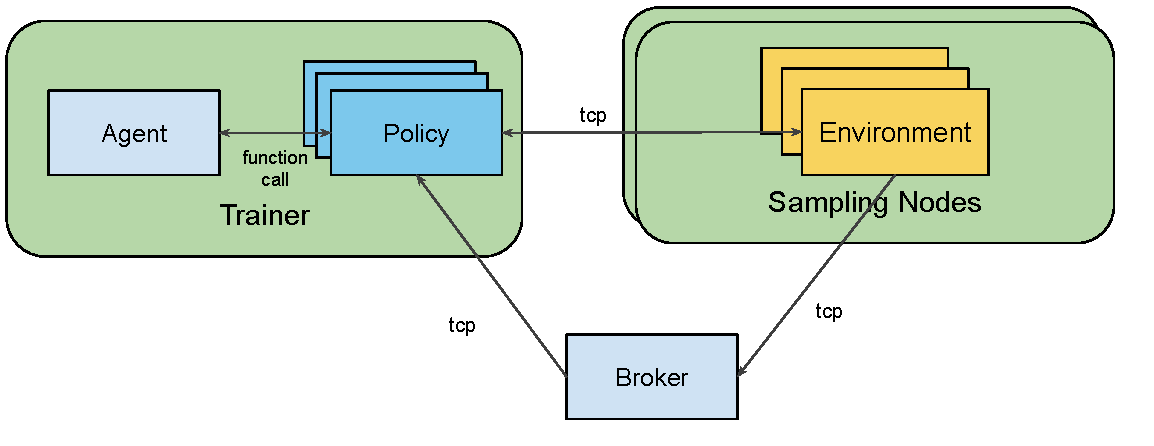
\includegraphics[width=0.7\textwidth]{images/Distributed-QBlade.pdf}
  \caption{A schema of the distribution framework. Environments can be placed on different nodes than the node the training is running on}
  \label{fig:distributed-framework}
\end{figure}

This asynchronous reset is the main idea constituting our framework for distributed wind turbine reinforcement learning \cite{westerbeckFrameworkDistributedWind2021}. Figure \ref{fig:distributed-framework} outlines this concept. Environments are process-separated from the sampling policy and communicate via tcp. This enables placement of environments on multiple sampling nodes, which can be different to the node of the sampling policy. The individual nature of the environments further allows them to reset asynchronously, as for the reset, no policy input is needed. The connection is established after a successful reset with the help of a \textit{broker} component, which keeps track of the state and tcp address of all environments and hands out a ready environment to requesting policies. 

It is possible to scale the amount of environments past the amount of sampling policies in our framework, effectively enabling a total speed-up factor up to the ratio of reset time to sampling time. As some simulation configurations need a reset time equal to the sampling time, we could measure a factor two speed-up over the default distributed sampling implementation by garage. All tcp connections are wrapped with ZeroMQ, enabling a fault-tolerant training process, and serialization is performed through protobuf, a high-speed and language agnostic serialization protocol.

Further improvements include changes to the multiprocessing sampler. The garage implementation offers an inefficient sampling stop condition. The sampler keeps starting new rollouts until the desired amount of environment interactions has been recorded. For example, if eight workers collect rollouts in parallel and seven of these finish, the stop condition has not been reached. Hence, all seven workers are instructed to collect another rollout. When the slowest worker finishes the first rollout shortly after, the stop condition is reached and sampling stops. Problematically, the seven other workers have already allocated an environment. They discart their allocation, and the environment has to reset. This behavior is acceptable for environments with short reset times, but for wind turbine environments with long reset times, this is a major performance loss. Changing this behavior has lead to another measured speed-up factor of almost two.

To perform grid searches, we investigated the hyperparameter tuning framework ray tune by \citet{liawTuneResearchPlatform2018}. Ray tune implements several sophisticated hyperparameter search algorithms and promises easy integration into any machine learning setup. However, we observed problematic behavior due to the fact that both ray tune and garage utilize the distributed python library ray. Ray spawns a number of components each time it is used, including a redis instance and several worker and watchdog processes. When combining the two frameworks and scaling them to a decent extent, the resulting utilization of unix processes and tcp ports exceeds the possibilities of the linux operating system on the cluster. The default reaction of linux is to fail the fork operation or socket allocation, which immediately crashes the training process and the involved ray worker. To make matters worse, ray workers are self-healing, means if a worker is missing, it is respawned immediately. In this case, this meant that the processes killed by the operating system would be restarted immediately by ray. We were unable to manually kill ray processes as fast as ray respawned them, normal interaction with the ray cluster was broken due to the tcp port exhaustion, and the operating system was unresponsive due to the accidental fork bomb. Hence, we implement our own grid search framework based on pythons inbuilt multiprocessing capabilities.
  

\subsection{Hyperparameters}
\label{section:approach-hyperparameters}

\begin{summary}
The choice of hyperparameters is a significant success factor to machine learning in general. This subsection presents a table of hyperparameters and describes our process of hyperparameter choice. In addition, we present the intuition behind hyperparameter effects for some hyperparameters. Because of space constraints, we can not include the entire experimentation performed to obtain these values. However, we include grid searches for a selection of hyperparameters in the results chapter.
\end{summary}

In Table \ref{table:hyperparameters}, hyperparameters and their default values for each wind scenario are listed. We require different hyperparameters for the different wind scenarios as the challenges associated with each scenario are different. The steady wind has a fully deterministic dynamic where subtle changes in the policy have a great impact, while the turbulent wind is dominated by the unpredictable nature of the wind inflow. These defaults form a basis for obtaining solid training results. When we deviate from these hyperparameters in the results section, we denote these deviations.

\newcommand\hparam[4]{#4 & $#1$ & #2 & #3  \\}
\begin{table}
  \centering
  \begin{longtable}{lccc}
    \toprule
    Description & Symbol & Steady & Turbulent \\
    \midrule
    \hparam{\targetupdate}{0.995}{0.995}{Smooth target update coefficient}
    \hparam{\gamma}{0.98}{0.99}{Discounting factor}
    \hparam{}{tanh}{tanh}{Activation function of the policy MLP}
    \hparam{}{256, 256}{256, 256}{Sizes of the hidden layers of the policy MLP}
    \hparam{}{tanh}{tanh}{Activation function of the Q function MLP}
    \hparam{}{256, 256}{256, 256}{Sizes of the hidden layers of the Q function MLP}
    \hparam{}{3e-5}{1e-5}{Learning rate of the policy}
    \hparam{}{3e-4}{1e-4}{Learning rate of the Q function}
    \hparam{\alpha_0}{0.05}{0.2}{Initial policy standard deviation}
    \hparam{\targetentropy}{-20}{-20}{Target entropy}
    \hparam{}{16000}{24000}{Number of environment interactions per epoch}
    \hparam{\lambdatraj}{2000}{2000}{Maximal trajectory rollout length}
    \hparam{}{200}{200}{Number of gradient descend steps per epoch}
    \hparam{}{256}{256}{Training batch size}
    \hparam{}{2e6}{2e6}{Maximum replay buffer size}
    \hparam{}{16e4}{16e4}{Minimal replay buffer size before commencing training}
    \hparam{\lambdaspat}{0.01}{0.2}{Spatial regularization coefficient}
    \hparam{\lambdatemp}{0.05}{0.2}{Temporal regularization coefficient}
    \hparam{\epsspat}{0.1}{0.1}{Spatial regularization standard deviation}
    % \hparam{\drrrcoeff}{0}{DR3 regularization coefficient}
    \hparam{\lambdapast}{6}{6}{Dilated past feeding steps}
    \hparam{\rcoleman}{2e-7}{2e-7}{Reward blade bending penalty}
    \hparam{\rconst}{1}{1}{Reward function constant offset}
    \hparam{\rcolemanact}{0}{0.02}{Reward pitch travel penalty}
    \hparam{}{$\pm$5}{$\pm$5}{Reward clipping range}
    \midrule
    \hparam{}{false}{true}{Allow $c_S$ action control}
    \hparam{\ipcplay}{$\pm$ 3}{$\pm$ 4}{IPC control play [deg]}
    \hparam{}{$\pm0.5$}{$\pm0.5$}{$\philead$ control play [rad]}
    \hparam{\tauhp}{$1/0.2$}{$1/0.2$}{Preprocessing high-pass filter tau}
    \hparam{\pitchmodelfreq}{$4\cpi$}{$4\cpi$}{Pitch actuator model frequency}
    \hparam{\pitchmodeldamp}{0.7}{0.7}{Pitch actuator model damping coefficient}

    \bottomrule
  \end{longtable}
  \caption{Table of hyperparameters with their symbol, default value and a description}
  \label{table:hyperparameters}
\end{table}

We found some hyperparameters to have a higher impact than others, among the most important ones being $\lambdatemp, \lambdaspat$. $\lambdatemp$ and $\lambdaspat$ modify the smoothness of the policy and have a high impact on pitch actuator wear. The smoother a policy is, the less pitch actuator wear it induces. Furthermore, they also have an impact on blade actuator wear, as a smoother policy also protects the blades, especially in the steady wind. 

$\gamma$ controls how strongly rewards far in the future are discounted, meaning how much influence they still have currently or how short-sighted optimization should be. In our case, this affects the relation of the reward function to the actual wear metrics. With a lower $\gamma$, the term minimizing pitch wear has a higher effect on pitch wear, while with a higher $\gamma$, the blade wear term is more effective. We credit this to the learnability of these functions, as blade wear is more difficult to learn than pitch wear. With a lower $\gamma$, the blade wear term is mainly noise, as most of the blade wear is induced by the wind. Only over longer periods of optimization, the difference another policy can have on blade wear becomes clear.

The number of environment interactions per epoch controls how often gradients are calculated. With 16000, we chose a value much higher than the \ac{SAC} defaults. While we found this to slightly hurt the number of epochs required to convergence, it did not significantly hurt final policy performance. With a higher number of environment interactions per epoch, we can parallelize the sampling process better. In this case, eight environments can sample in parallel, which results in a drastic reduction in wall-clock time. Further increasing the amount of steps per epoch yielded performance improvements that did not justify the additional compute budget anymore.

Initial policy standard deviation (also called initial temperature coefficient) $\alpha_0$ and target entropy $\targetentropy$ relate to the option of \ac{SAC} to control entropy in the maximum-entropy RL setting. During training, $\alpha$ will slowly approach $\targetentropy$ in an exponential decay pattern. For the wind turbine, choosing a low $\targetentropy$ means the policy will have minimal noise at the end of the training process. Some noise is required to ensure exploration, especially at the beginning of the training, so the starting entropy is a little higher. We tuned both parameters to the lower limit that would still allow stable training.

The activation functions are specified to be ReLU in the \ac{SAC}-paper, but we use tanh in our work. The difference between the two is minimal, but tanh yields slightly smoother policies in our experiments. As the networks are relatively shallow, typical problems with sigmoid-like activations like vanishing gradients on saturated activations or activation drift do not play out detrimental.

The size of the neural networks specifies the potential to learn complex functions. More parameters generally mean more difficult functions can be learned. In general machine learning, the number of parameters in a neural network can be used to control the bias-variance trade-off. In reinforcement learning, the bias-variance trade-off is not a big concern yet, as biases induced through the Bellman backup or other training techniques usually exceed approximation errors due to underparametrization \cite{fujimotoAddressingFunctionApproximation2018}. Consequently, minimizing bias is the primary aim, and the downside of high-variance estimators can be ignored by not benchmarking generalization \cite{cobbeQuantifyingGeneralizationReinforcement2019}. For more complex types of neural networks such as convolutional networks, a higher number of layers boosts training performance, but for a \ac{MLP}, the number of layers does not matter. Given enough neurons per layer, any function can be approximated with just two layers. With these considerations in mind, we found two layers with 256 neurons to work well; adding more neurons did not improve performance.

The training batch size is another parameter that is used to control the bias-variance trade-off in traditional machine learning. The smoothing effect of high batch sizes can be used to limit variance while loosing fine fit. Furthermore, high batch sizes improve GPU efficiency. Our cluster does not have GPUs and the bias-variance trade-off is not a major concern, so we utilize the default batch size from \ac{SAC}.

The learning rate is a parameter, which has a major impact in supervised learning. It dictates how far to make a gradient step, with too low values resulting in long trainings and high susceptibility to local maxima, and too high values in loss explosions and coarse fit. In reinforcement learning, a non-stationary quantity is subject to optimization. The Q-function targets change with policy performance and Q-function fit, hence a complex interaction of policy and Q-networks emerges, which makes the choice of learning rate non-trivial. \citet{kakadeNaturalPolicyGradient2001} prove that second-order optimization over the environment dynamics can find a sensible step size for each gradient, however \ac{SAC} uses first-order optimization only. Resultingly, the learning rate has to be sufficiently small to avoid catastrophic steps and detrimental interactions between policy and Q optimization. Furthermore, the dynamic between policy and Q-function is complex to control. We found a policy learning rate one magnitude smaller than the Q learning rate to stabilize trainings, as the Q estimates have time to settle to the current policy performance before the policy changes too drastically.

Finding the best hyperparameters for a machine learning algorithm is a non-trivial task, and automatizing this task forms a separate field in machine learning called \textit{AutoML} \cite{hutterAutomatedMachineLearning2019}. We chose to optimize our hyperparameters through \textit{grid search}, which means to run a full training for every sensible combination of hyperparameters. As we lack the computation resources to perform a full grid search over all hyperparameters, we pair grid searches over small subsets of the hyperparameter space with \textit{grad student descend} \cite{gencogluHARKSideDeep2019}, a methodology where a student tries hyperparameter subsets until it works.


\subsection{Evaluation Methodology}
\label{section:approach-evaluation-methodology}

\begin{summary}
This subsection describes the evaluation procedures and metrics used, comparison baselines, and the exact procedure for calculating metrics. Our baselines are a \ac{CPC} and a \ac{IPC} control strategy, with our main metric being DELs, a metric for component wear. 
\end{summary}

\subsubsection{Baselines}

We use two validated controllers as a reference baseline. One is a \acf{CPC} as described in \cite[Section 3.2.1]{perez-beckerImplementationValidationAdvanced2021}. It integrates state-of-the-art features such as gain scheduling, notch-filtering drivetrain eigenfrequencies, and techniques to prevent integrator saturation. Its parameters were tuned to the IEA 10MW turbine by an expert for wind turbine control. Furthermore, we use a second baseline which implements an \acf{IPC} as described in \cite[Section 3.2.2]{perez-beckerImplementationValidationAdvanced2021}. We outline the properties of this strategy in our background Section \ref{section:background-ipc}. Similar to the \ac{CPC}, parameters were tuned to the IEA 10MW turbine by an expert for wind turbine control.

\subsubsection{Procedures}

Garage offers inbuilt evaluation capabilities. After each epoch, the algorithm can be evaluated in a separate evaluation environment. This inbuilt evaluation phase offers no distribution option, and it is difficult to extract and save collected evaluation rollouts for further inspection. We implement a separate evaluation phase which runs in a dedicated Slurm job. The configuration of our evaluation environments is different to the training configuration. Hence, separating the evaluation phase to another job results in better hardware utilization, as only the type of environments which is in use is spawned.

While our training takes place in randomized environments, we utilize deterministic settings for the simulation in the evaluation phase. For tracking our training progress, each checkpoint is evaluated in eight deterministic environments. From this, metrics are accumulated to form training plots. For a detailed evaluation of a single checkpoint, we utilize a higher number of deterministic environments. In the steady wind setting, we evaluate the wind range in 0.1 m/s steps. In the turbulent setting, we evaluate in 0.2 m/s steps with eight turbulence seeds for each wind speed. To allow for a direct comparison of policy performance, the baseline \ac{CPC}, the baseline \ac{IPC}, and our neural controller are run on each of the environments.

We observed slightly better results with deterministically evaluated policies compared to using the stochastic policy directly. Hence, we evaluate our trained policies deterministically for the entire evaluation: $\pi_{\text{det}}(s) = \argmax_{a} \pi(a|s)$. As the output of the policy is a multivariate Gaussian, the argmax operation is implemented by taking the mean of the Gaussian as action output. Through both a deterministic policy and a deterministic environment, the evaluation rollouts are deterministic and can be compared directly. Unless stated otherwise, we utilize the highest performing policy of a training run, which not necessarily the last iteration.

As recommended in \citet{agarwalDeepReinforcementLearning2022}, we use the \acf{IQM} method for mean estimations that are robust to outliers in most of this work. The \ac{IQM} of a set of values is computed by discarting the lowest 25\% and highest 25\% of all elements and computing the arithmetic mean across the remaining elements. For example, the values $\{1, 1.1, 1.3, 4.7\}$ are pruned to $\{1.1, 1.3\}$ and then averaged to an IQM of 1.2. The values can be of any metric for which a traditional arithmetic mean can be calculated.

\subsubsection{Metrics}

While reward is the quantity subject to optimization, we utilize further metrics to improve interpretability of our results.

As additional evaluation metrics, we calculate \acp{DEL} as outlined in Section \ref{section:damage-equivalent-loads} for \ac{BRBM} and for pitch actuation. For brevity, we denote \ac{bDEL} as the \ac{DEL} metric for \ac{BRBM} and \ac{pDEL} for pitch actuation. We use the python framework \textit{rainflow} for rainflow calculation, which we found to deliver reasonably close results to those of \textit{Crunch} \cite{buhlCRUNCHUSERGUIDE2001}, a widely validated and adopted tool which supports Rainflow counting. We bin to n=128 bins, cohering to the default settings of Crunch. For calculating \acp{bDEL}, we use a Wöhler exponent $\woehler = 10$ which is typical for glass fiber and a \ac{DEL} frequency $\fdel = 1$ Hz. Furthermore, we average \acp{bDEL} of the three individual blades into one value. The resulting formula is shown in Equation \ref{eq:bdel}:

\begin{equation}
  \bdel = \frac{1}{3} \sum_{i \in {1,2,3}}(\del(\trajectory_{\soopbend_i}, \woehler=10, \fdel=1))
  \label{eq:bdel}
\end{equation}

where $\trajectory_{\soopbend_i}$ denotes the bending moment signal of blade $i$ along the entire trajectory $\trajectory$. For \acp{pDEL} $\pdel$, the DEL metric of the pitch signals, we use $\woehler = 1$ and $\fdel = 1$ Hz. We average the resulting \ac{pDEL} values across all blades, as in Equation \ref{eq:pdel}:

\begin{equation}
  \pdel = \frac{1}{3} \sum_{i \in {1,2,3}}(\del(\trajectory_{\spitchx_i}, \woehler=1, \fdel=1))
  \label{eq:pdel}
\end{equation}

with $\trajectory_{\spitchx_i}$ denoting the pitch actuation signal of blade $i$ along the trajectory. To calculate an improvement, we divide the reinforcement learning results by the results obtained by running the baseline \ac{IPC} on the same simulation setting: $\delrel = \frac{\del_{rl}}{\del_{ipc}}$. Values of $\delrel<1$ mean the learnt policy performs better than the baseline \ac{IPC}, in the sense of creating less \ac{DEL}. 

% Finally, a weighted DEL metric \textit{wDEL} which combines the relative pitch \ac{pDEL} $\pdelrel$ with the relative blade \ac{DEL} $\bdelrel$ can be computed as $\wdel(\pbtrade) = \pbtrade \bdelrel + (1-\pbtrade) \pdelrel$. The pitch-blade trade-off factor $\pbtrade \in [0,1]$ determines the relative importance of reducing blade bendings versus reducing pitch actuation. This trade-off factor is to be determined for each turbine, and is affected by a variety of engineering constraints such as parts cost, lifetime, and wear resilience. A factor $\pbtrade > 0.5$ means lowering $\pdel$ is more important than lowering $\bdel$, and vice versa. Hence, an RL policy, which reduces bending moments while increasing pitch actuation, is still evaluated as an improvement over the baseline if the pitch actuation increase is outweighed.

In the turbulent wind setting, extreme loads also play a role. In contrast to fatigue loads, the number of cycles can be minimal to cause damage to the blade. Albeit DELs capture the full load range, the metric exhibits inaccuracies on extreme values. Hence, we quantify them separately with the 99\% quantile value of blade bending moments. The pitch actuator does not require an extreme load analysis, as the pitch actuator is more susceptible to wear through high and fast pitch travel than to high pitching amplitude.

To qualitatively analyze behavior, we use the visualization tool \acf{PSD} plot. These plots show the spectral activity of a time series. They have the frequency spectrum on the x-axis and the intensity of activity on that frequency on the y-axis. In our work, we utilize log-scales for the y-axis to facilitate readability. They are computed by Fourier-transforming the time series and then summing the frequency contents of the Fourier-transformed signal across the time axis. A pure sine wave would show as a single excited frequency in the Fourier-transformed signal, as a horizontal line in a spectogram, and as a single peak in a \ac{PSD} plot. If there are peaks on exact multiples of a frequency, these multiples are called \textit{harmonic frequencies}.
